\chapter{Theory}
\label{c:theory}

\section{Standard Model}

The standard model (SM)~\cite{Glashow:1961tr,PhysRevLett.19.1264,Salam:1968rm,DGriff} is a theory which describes the elementary particles and their interactions. Matter consists of six quarks and six leptons, each of which has an anti-particle with the same mass and opposite-sign charge. They are organised into three generations each of which contains heavier particles than the last, as seen in Table~\ref{table:SMmatter}. All of the normal matter in the universe is made up of particles from the first generation, ie.~up and down quarks make up protons and neutrons, and combined with electrons they form atoms. 

The leptonic sector consists of charged leptons, which can interact via the electromagnetic and weak forces, and neutrinos, which interact via the weak force only. The neutrinos are assumed to be massless in the standard model however observations of neutrino oscillations have revealed that neutrinos have mass~\cite{PhysRevC.88.025501}.

\vspace{0.8cm}
\begin{table}[ht!]
\centering
\caption{Quarks and leptons}
\label{table:SMmatter}
\footnotesize
\begin{tabular}{|c|l|l|l|l|l|l|}
\hline
\multirow{2}{*}{Generation} & \multicolumn{3}{c|}{Quarks}                             & \multicolumn{3}{c|}{Leptons}              \\ \cline{2-7} 
                            & Flavour & Charge & Mass (MeV)                           & Flavour      & Charge & Mass (MeV)        \\ \hline
\hline

\multirow{2}{*}{I}          & u       & 2/3    & $2.2^{+0.6}_{-0.4}$                  & e            & -1     & 0.511             \\
                            & d       & -1/3   & $4.7^{+0.5}_{-0.4}$                  & $\nu_{e}$    & 0      & $<2\times10^{-6}$ \\ \hline
\multirow{2}{*}{II}         & c       & 2/3    & $(1.27\pm 0.03)\times10^{3}$         & $\mu$        & -1     & 105.66            \\
                            & s       & -1/3   & $96^{+8}_{-4}$                       & $\nu_{\mu}$  & 0      & $<0.19$           \\ \hline
\multirow{2}{*}{III}        & t       & 2/3    & $(173.21\pm0.51\pm0.71)\times10^{3}$ & $\tau$       & -1     & $1776.86\pm0.12$  \\
                            & b       & -1/3   & $(4.18^{+0.04}_{-0.3})\times10^{3}$  & $\nu_{\tau}$ & 0      & $<18.2$           \\ \hline
\end{tabular}
\end{table}

Quarks interact via the electromagnetic, weak or strong force. Each quark has an electric charge, as seen in Table~\ref{table:SMmatter}, and carries a colour charge of red, green or blue, where all three colours combined can form a colour-singlet state. A combination of quarks with a colour and its anti-colour can also form a colour-singlet state. The theory of colour confinement means that quarks can only be found in colour-singlet states such as in baryons or mesons. 

Finally, the force carriers consist of gauge bosons of integer spin, as seen in table~\ref{table:SMbosons}. Photons and Z bosons can mediate neutral electroweak interactions whereas W bosons can mediate charged electroweak interactions. The gluons mediate the strong interaction and occur with 8 different types of colour charge which will be described in section~\ref{subsec:QCD}. 
% The Graviton is hypothesised to carry the gravitational force but there is as yet no evidence to support this hypothesis.
\begin{table}[ht!]
\centering
\caption{Gauge bosons}
\footnotesize
\label{table:SMbosons}
\begin{tabular}{|l|l|l|l|l|l|}
\hline
Gauge boson                       & Force           & Charge & Mass (GeV) & Spin & Range (m)  \\ \hline \hline
Photon ($\gamma$)                 & electromagnetic & 0      & 0          & 1    & $\infty$   \\ \hline
W$^{\pm}$                         & weak            & $\pm1$ & $80.385\pm0.015$           & 1    & $10^{-18}$ \\ \hline
Z                                 & weak            & 0      & $91.1876\pm0.0021$           & 1    & $10^{-18}$ \\ \hline
gluon                             & strong          & 0      & 0          & 1    & $10^{-15}$ \\ \hline
% Graviton\footnote{hypothesised} & gravitational   & 0      & 0          & 2    & $\infty$   \\ \hline
\end{tabular}
\end{table}

The discovery of the Higgs boson in 2012~\cite{Higgs2012observation,Aad:2012tfa,Aad:2015zhl}. completed the standard model with an explanation of how the fundamental particles acquire mass via the electroweak symmetry breaking mechanism.\\

The SM is a gauge theory based on the symmetry group SU(3)~x~SU(2)~x~U(1), which is a combination of the electroweak interactions based on the SU(2)~x~U(1) symmetry group and the strong interaction which is based on the SU(3) group.

The SM will now be described in more detail.

\subsection{Electroweak theory}

\subsubsection{Quantum Electrodynamics}
\label{subsec:QED}

Quantum Electroydynamics is an Abelian gauge theory based on the U(1) symmetry group. Figure~\ref{fig:QEDvertex} shows the elementary QED vertex where a charged particle (charged lepton or quark) and charged anti-particle interact with a photon, where the convention used in this thesis is that time flows from left to right. However, these diagrams may be rotated as long as they conserve energy. Hence, this vertex can describe particle-anti-particle annihilation into a photon, a photon pair-producing an particle-anti-particle pair, an particle emitting a photon or a anti-particle emitting a photon depending on the orientation of the diagram. QED interactions conserve lepton or quark flavour.


\begin{figure}[ht!]
\begin{center}
    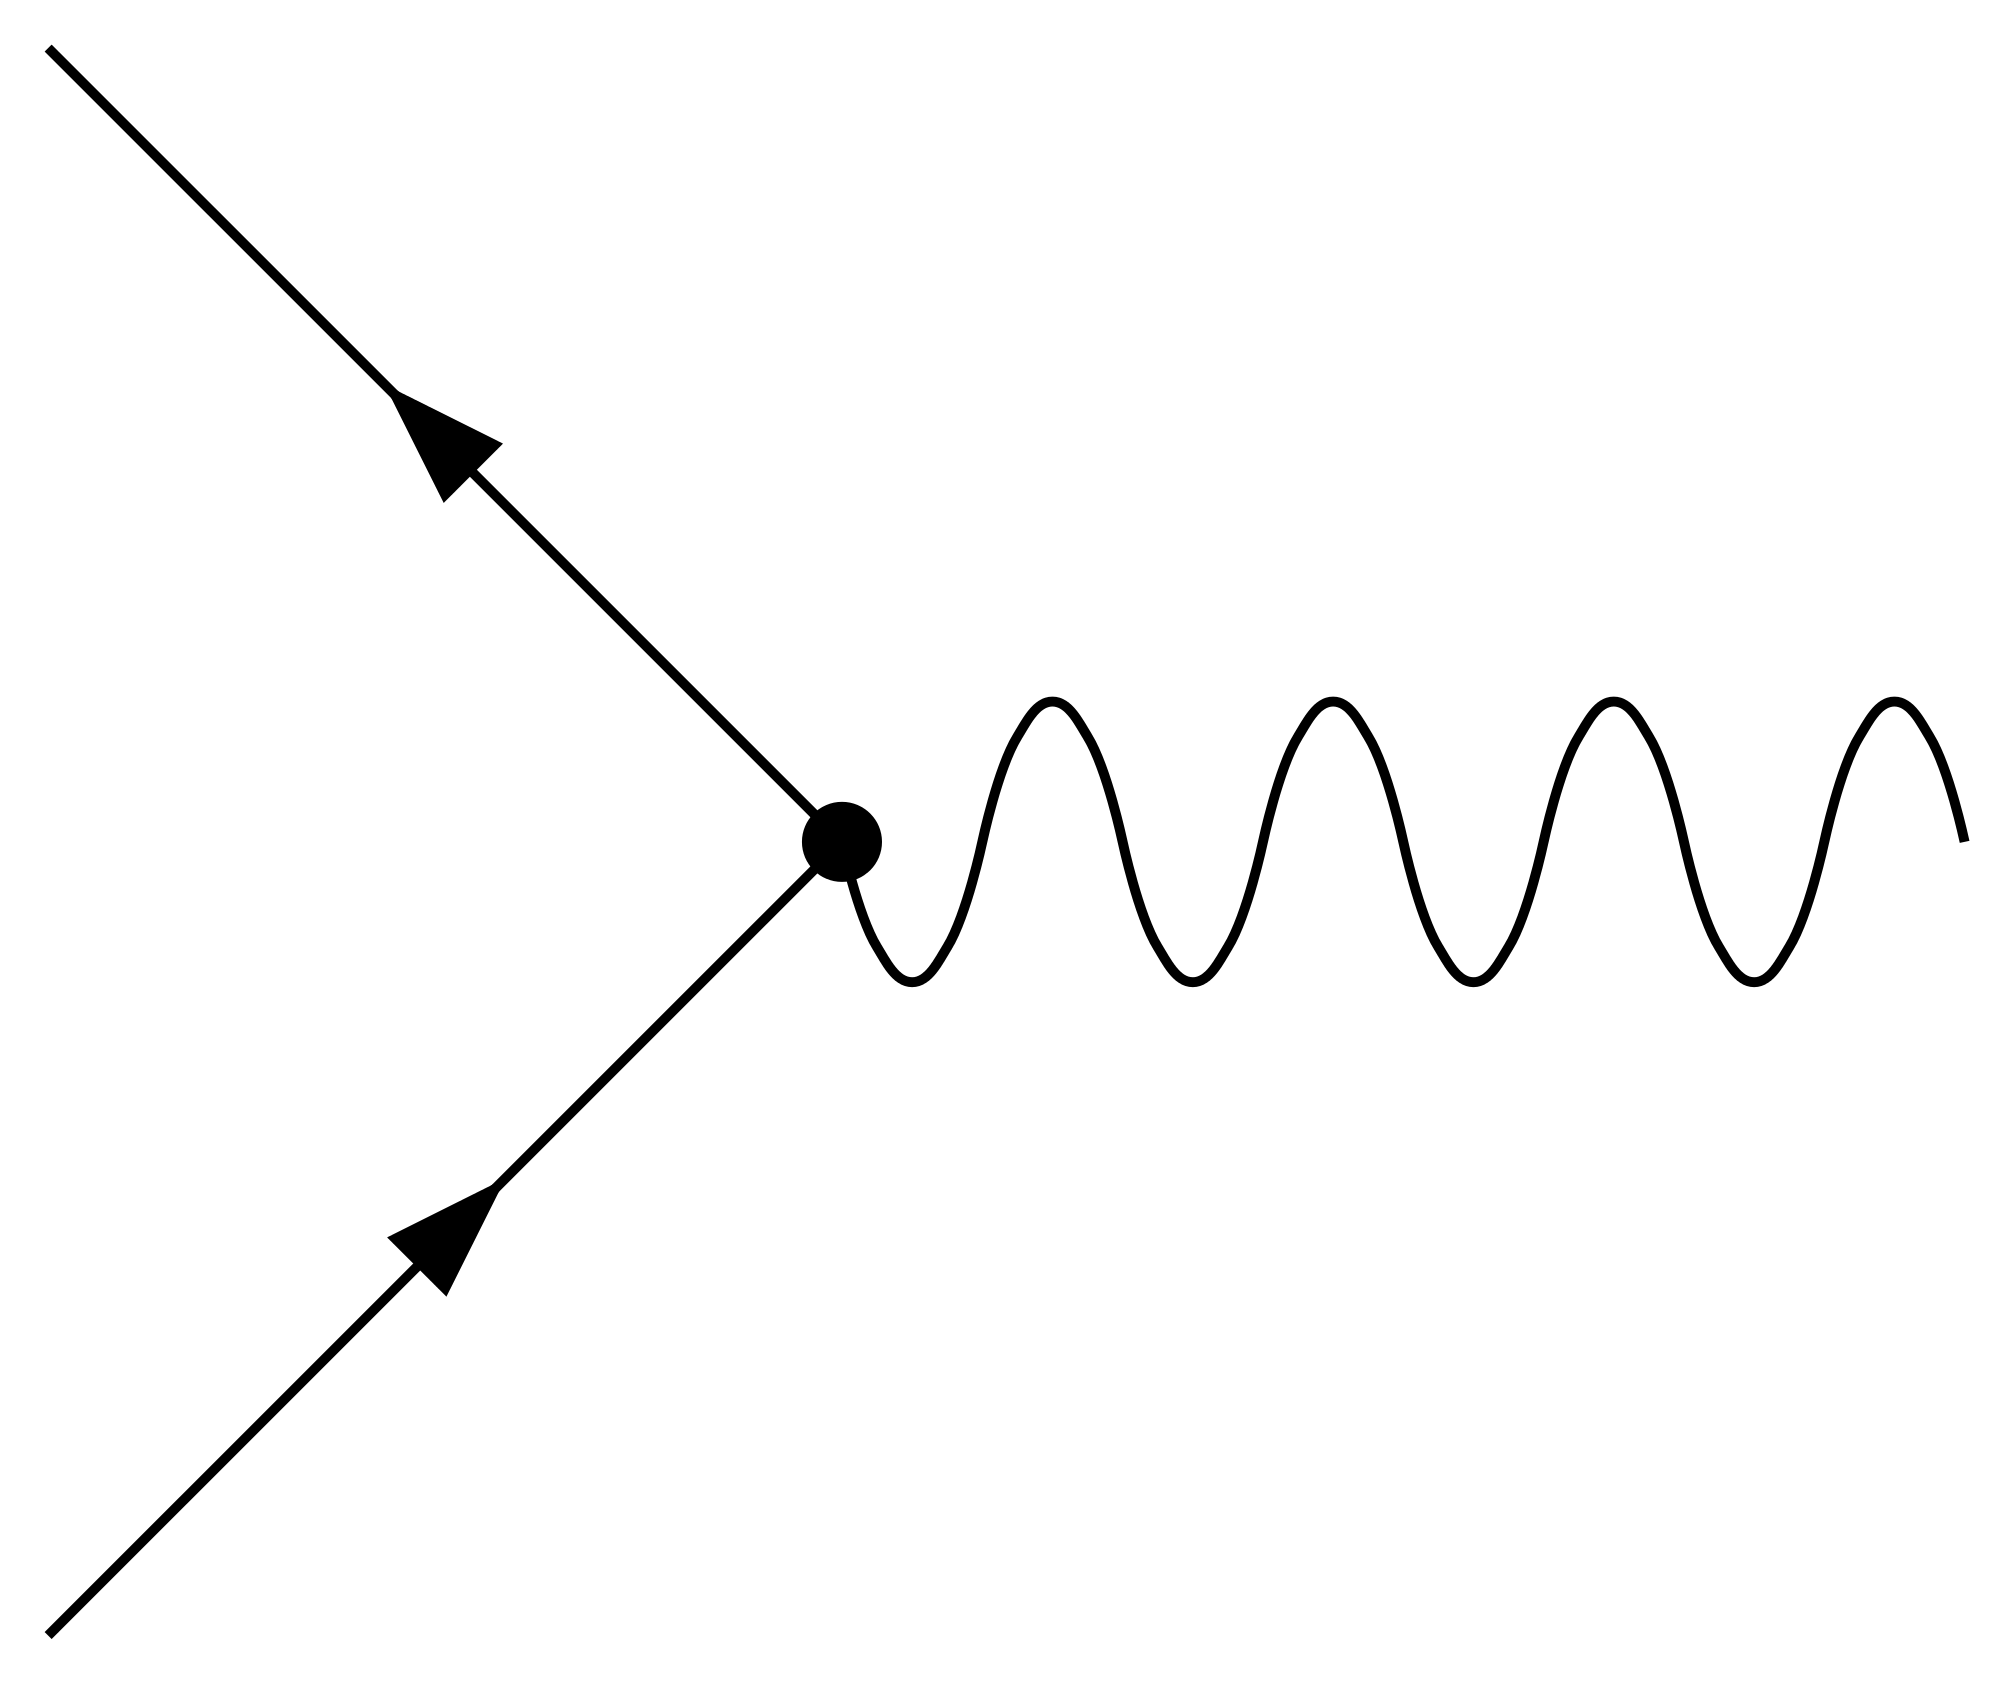
\includegraphics[width=0.35\textwidth]{images/Theory/QEDvertex.png}
    \caption{Elementary QED vertex}
    \label{fig:QEDvertex}
\end{center}
\end{figure}

% This diagram alone cannot occur as it violates conservation of energy but it can be used to build a full Feynman diagram for a particle physics process.
The QED Lagrangian can be found in Eq.~\ref{eqn:QEDL} with $D_{\mu}$ representing the covariant derivative which is defined as $D_{\mu} = \partial_{\mu} + iqA_{\mu}$. 
\begin{equation}
\mathcal{L} = \overline{\psi}\left(i\gamma^{\mu}D_{\mu}-m\right)\psi - \frac{1}{4}F_{\mu\nu}F^{\mu\nu}
\label{eqn:QEDL}
\end{equation}
Here $q$ represents the charge of the particle and $A^{\mu}$ is the massless field of the electromagnetic four-potential. Dirac Lagrangian is manifestly invariant to global phase transformations $\psi \rightarrow e^{i\theta} \psi$. The supplementation by $iqA_{\mu}$ is required to make the Lagrangian invariant to local phase transformations $\psi \rightarrow e^{i\theta(x)} \psi$ where $A_{\mu}$ transforms as $A_{\mu} \rightarrow A_{\mu} + \partial_{\mu}\theta(x)$. Hence, the QED Lagrangian is gauge invariant under U(1) phase transformations, where U(1) is the unitary group of complex numbers. 

The mass of the particle is represented by $m$ and $F_{\mu\nu} = \partial_{\mu}A_{\nu} - \partial_{\nu}A_{\mu}$ is the electromagnetic field tensor.

Application of the Euler-Lagrange equations leads to the derivation of the Dirac Equation shown in Eq.~\ref{Eqn:Dirac}.
% , where $J_{\mu} = \overline{\psi}\gamma_{\mu}\psi$.

\begin{equation}
i\gamma^{\mu }\partial _{\mu }\psi -m\psi - iq\gamma^{\mu }A_{\mu} = 0
\label{Eqn:Dirac}
\end{equation}

The Dirac equation describes the motion for spin-1/2 particles with mass, ie. quarks and charged leptons. From this equation the Feynman rules for QED can be derived. These rules allow the computation of a number, known as the \emph{amplitude}, for each Feynman diagram. The sum total of the amplitudes for all diagrams which represent a particular process can be summed to produce the probability or \emph{cross section} for that process to occur.

In QED the vacuum acts like a dielectric medium which produces electron-positron pairs where the virtual electron is attracted to positive charges and the virtual positron is repelled (and vice versa for negative charges). This vacuum polarisation partially screens the charged particle and effectively reduces its field. However at short distances, the effective charge increases as the screening reduces.
% \textbf{Effective coupling}

\subsubsection{Weak interactions}

The charged weak interaction is the only interaction where a flavour changing process can occur. The diagram of weak nuclear decay in Fig.~\ref{fig:QEDvertex} illustrates the W boson's interaction with different flavour quarks and leptons. The are two W bosons, one of positive and one of negative charge, W$^{\pm}$.


\begin{figure}[ht!]
\begin{center}
    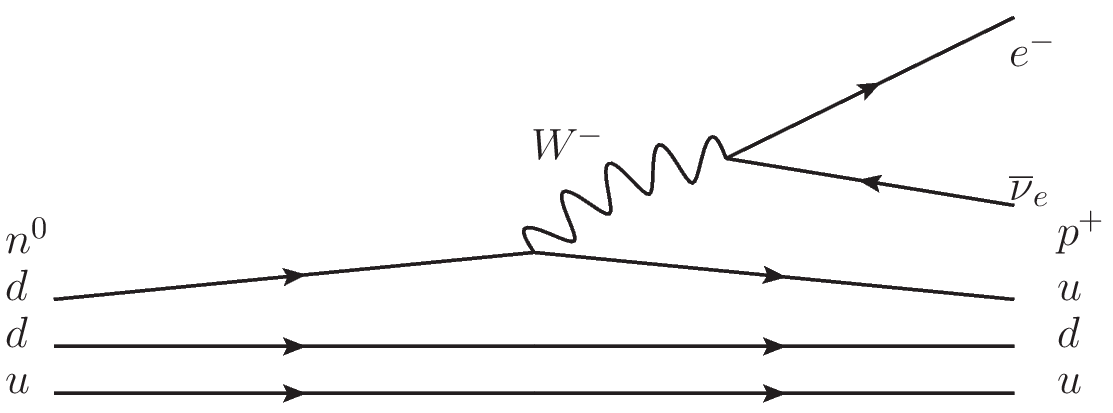
\includegraphics[width=0.65\textwidth]{images/Theory/weakDecay.png}
    \caption{Weak nuclear decay of neutron to proton}
    \label{fig:QEDvertex}
\end{center}
\end{figure}

The neutral weak interaction is mediated by Z bosons which can interact with any quark or lepton as long as the flavour is conserved at the vertex.

As the weak force bosons are massive, this means that weak decays are much slower than decays via electromagnetism for instance. This means that particles that can only decay via the weak force have longer lifetimes. 

The weak force only interacts with chirality left-handed (right-handed) particles (anti-particles), ie. particles where the spin is (anti-)aligned with the momentum direction. The charge for weak interaction is \emph{weak isospin} ($I_{3}$) which is $\pm1/2$ for left-handed fermion, $\pm1$ for W$^{\pm}$ and zero otherwise.

Weak interactions are the only interactions known to violate parity conservation, which was hypothesised by Yang and Lee~\cite{PhysRev.104.254} and experimental validated by Wu in 1957~\cite{PhysRev.105.1413}. It was later discovered that weak interactions also violate the combined charge-parity (CP) symmetry~\cite{Cronin2012,PhysRevLett.13.138}.

\subsubsection{Electroweak Unification}

Glashow~\cite{Glashow:1961tr}, Weinberg~\cite{PhysRevLett.19.1264} and Salam~\cite{Salam:1968rm} formulated the unification of the weak and electromagnetic forces combined in the SU(2)~x~U(1) gauge group. They are hypothesised to merge into one electroweak force above the unification energy of $\approx 100$~GeV. The theory contains four gauge bosons: three W bosons W$_{a}~(a=1,~2,~3)$ and one B boson. Weak hypercharge is defined as $Y_{W} = 2(Q-I_{3})$ and it is $Y_W$ which is the generator of the U(1) component of the electroweak gauge group, which is mediated by the B boson. Equation~\ref{eq:EWK_L} shows the Lagrangian for electroweak interactions where it can be seen that the left-handed fields, contained in the doublet $\psi_{L}$, couple to the W and B bosons and the right-handed fields, $\psi_{R}$, couple to the B boson only. The generators of SU(2) component are ${\bf T} = \boldsymbol{\sigma}/2$ where $\boldsymbol{\sigma}$ are the Pauli matrices.
\begin{equation}
\label{eq:EWK_L}
\begin{split}
\calL_\textrm{EWK} & = \bar{\psi}_L \gamma^\mu ( i\partial_\mu  - g \mathbf{T} \cdot \mathbf{W}_\mu - \frac{g'}{2} Y_{W}
B_\mu) \psi_L + \\ & + \bar{\psi}_R \gamma^\mu (i \partial_\mu - \frac{g'}{2} Y_{W} B_\mu) \psi_R -
\frac{1}{4}\mathbf{W}_{\mu\nu} \mathbf{W}^{\mu\nu} -\frac{1}{4}B_{\mu\nu} B^{\mu\nu},
\end{split}
\end{equation}

\begin{equation*}
\psi_L = \twovector{\psi^u_L}{\psi^d_L}, \twovector{\psi^\nu_L}{\psi^l_L},~~\psi_R=~\psi_R^u,~\psi_R^d,~\psi_R^l
\end{equation*}

The spontaneous symmetry breaking mechanism proposed by Brout, Englert~\cite{PhysRevLett.13.321} and Higgs~\cite{PhysRevLett.13.508} results in the linear combination of these 4 bosons into the four more familiar gauge bosons from Table~\ref{table:SMbosons}, W$^{\pm}$, Z and the photon ($\gamma$) as shown in Eqs.~\ref{eqn:Zgamma} \&~\ref{eqn:Wpm}, where $\theta_{W}$ is the weak mixing angle.
\begin{equation}
\label{eqn:Zgamma}
{\begin{pmatrix}
\gamma \\
\textrm{Z} 
\end{pmatrix}}
=
{\begin{pmatrix}
\cos\theta_{W} & \sin\theta_{W} \\
-\sin\theta_{W} & \cos\theta_{W} 
\end{pmatrix}}
{\begin{pmatrix}
\textrm {B} \\
\textrm{W}_{3}
\end{pmatrix}}
\end{equation}

\begin{equation}
\label{eqn:Wpm}
\textrm{W}^{\pm}=\frac{1}{\sqrt{2}}\left(\textrm{W}_{1}\mp i\textrm{W}_{2}\right)
\end{equation}

% Equation~\ref{eqn:EWL} shows the electroweak Lagrangian where $\mathcal{L}_{K}$ gives the kinetic term, $\mathcal{L}_{N}$ gives the neutral interactions and $\mathcal{L}_{C}$ the charged interactions. $\mathcal{L}_{H}$ gives the Higgs three and four point self-interactions and  $\mathcal{L}_{HV}$ gives the Higgs interactions for vector bosons.  $\mathcal{L}_{WWV}$ ($\mathcal{L}_{WWVV}$) gives the three (four) point interactions of the vector bosons and $\mathcal{L}_{Y}$ gives the Yukawa couplings between the Higgs field and the fermions.

% \begin{equation}
% \label{eqn:EWL}
% \mathcal{L}_{EW} = \mathcal{L}_{K} + \mathcal{L}_{N} + \mathcal{L}_{C} + \mathcal{L}_{H} + \mathcal{L}_{HV} + \mathcal{L}_{WWV} + \mathcal{L}_{WWVV} + \mathcal{L}_{Y}
% \end{equation}

% and $\psi_L$ and $\psi_R$ are summed over all possibilities shown in Equations~\ref{eq:lepton_EWK_fields} and
% \ref{eq:quark_EWK_fields}.

% The Yukawa couplings, which describe the couplings between dirac fields and a scalar field, 

After electroweak symmetry breaking where the Higgs boson gets a vacuum expectation value, the electroweak Lagrangian changes into the form in Eq.~\ref{eqn:EWL2} which is described in Ref~\cite{Pich:2005mk}. Here $\mathcal{L}_{K}$ gives the kinetic term, $\mathcal{L}_{N}$ gives the neutral interactions and $\mathcal{L}_{C}$ the charged interactions. $\mathcal{L}_{H}$ gives the Higgs three and four point self-interactions and $\mathcal{L}_{HV}$ gives the Higgs interactions for vector bosons. The term $\mathcal{L}_{WWV}$ ($\mathcal{L}_{WWVV}$) gives the three (four) point interactions of the vector bosons and $\mathcal{L}_{Y}$ gives the Yukawa couplings between the Higgs field and the fermions.

\begin{equation}
\label{eqn:EWL2}
\mathcal{L}_{EW} = \mathcal{L}_{K} + \mathcal{L}_{N} + \mathcal{L}_{C} + \mathcal{L}_{H} + \mathcal{L}_{HV} + \mathcal{L}_{WWV} + \mathcal{L}_{WWVV} + \mathcal{L}_{Y}
\end{equation}

The charged current interaction is particularly interesting for the W decays from top quarks. It is described by the term in Eq.~\ref{eqn:CCint}. 

\begin{equation}
\label{eqn:CCint}
\mathcal{L}_{C} = \frac{g}{\sqrt{2}} i\bar{\psi_{L}} \gamma^{\mu} \partial_{\mu} \psi_{L}
\end{equation}
\begin{equation*}
\psi_L = \twovector{u_L}{{d'}_L}, \twovector{\nu_L}{l_L}
\end{equation*}

Here ${d'}_L = V_{CKM}~d_L$.


The CKM matrix, also known as the \emph{quark mixing matrix}, is a unitary matrix which describes the strength of the couplings for weak decays and is shown in Eq.~\ref{eqn:CKM1}. 
\begin{equation}
\label{eqn:CKM1}
{\begin{pmatrix}
d^{\prime }\\
s^{\prime }\\
b^{\prime }
\end{pmatrix}}
=
{\begin{pmatrix}
V_{ud}&V_{us}&V_{ub}\\
V_{cd}&V_{cs}&V_{cb}\\
V_{td}&V_{ts}&V_{tb}
\end{pmatrix}}
{\begin{pmatrix}d\\s\\b
\end{pmatrix}}
\end{equation}
The probabilities for the up-type quarks to couple to down-type quarks are given in Eq.~\ref{eqn:CKM2}.
\begin{equation}
\label{eqn:CKM2}
{\begin{pmatrix}
|V_{ud}|&|V_{us}|&|V_{ub}|\\|V_{cd}|&|V_{cs}|&|V_{cb}|\\|V_{td}|&|V_{ts}|&|V_{tb}|
\end{pmatrix}}
=
{\begin{pmatrix}0.97417\pm 0.00021 & 0.2248\pm 0.0006 & 0.00409\pm{0.00039}\\
0.220\pm 0.005 & 0.995\pm 0.016 & 0.0405\pm{0.0015}\\
0.0082\pm{0.0006} & 0.040\pm{0.0027}&1.009\pm0.031
\end{pmatrix}}
\end{equation}



\subsection{Quantum chromodynamics}

Quantum chromodynamics (QCD) is a non-Abelian gauge theory based on the SU(3) symmetry group that describes the strong interactions between quarks and gluons. Quarks and gluons carry colour charge. Each (anti-)quark will carry one of \\(anti-)~red, (anti-)~green or (anti-)~blue colour charge whilst there are 8 types of gluon which exist in a superposition of colour-anti-colour states. One of the elementary QCD vertices is shown in Fig~\ref{fig:QCDvertex} where two quarks couple to a gluon. There are also three and four-point interactions between gluons.
\label{subsec:QCD}
\begin{figure}[ht!]
\begin{center}
    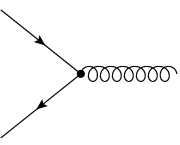
\includegraphics[width=0.35\textwidth]{images/Theory/QCDvertex.png}
    \caption{A elementary QCD vertex}
    \label{fig:QCDvertex}
\end{center}
\end{figure}


Equation~\ref{eqn:QCDL} gives the QCD lagrangian, $\mathcal{L}_{\textrm {QCD}}$ , where $G_{\mu \nu }^{a}=\partial _{\mu }{\mathcal {A}}_{\nu }^{a}-\partial _{\nu }{\mathcal {A}}_{\mu }^{a}+gf^{abc}{\mathcal {A}}_{\mu }^{b}{\mathcal {A}}_{\nu }^{c}$ is the gluon field strength tensor and $f^{abc}$ are the structure constants of SU(3).
\begin{equation}
    \label{eqn:QCDL}
{\mathcal {L}}_{\mathrm {QCD} }={\bar {\psi }}_{i}\left(i(\gamma ^{\mu }D_{\mu })_{ij}-m\,\delta _{ij}\right)\psi _{j}-{\frac {1}{4}}G_{\mu \nu }^{a}G_{a}^{\mu \nu }
\end{equation}

\textbf{Asymptotic freedom and colour confinement}\\
Quark-anti-quark loops lead to screening of the quark colour charge, however gluon loops contribute the opposite by `anti-screening'. It was found that in any theory with $11n>2f$, where $n$ is the number of colours and $f$ is the number of quark flavours, the coupling constant, $\alpha_{S}\left( |q^{2}| \right)$, will decrease with increasing energy, q$^{2}$~\cite{PhysRevLett.30.1343,PhysRevLett.30.1346}. This is known as \emph{asymptotic freedom} as the quarks inside hadrons effectively act like free particles. This is in contrast to QED where there is no `anti-screening' effect.

% \begin{equation}
% \label{eqn:alphaSQCD}
% \alpha_{S}\left( |q^{2}| \right) = \frac{\alpha_{S}\left( \mu^{2} \right)} {1 + \left[ \alpha_{S}\left( \mu^{2} \right)/12\pi \right]\left( 11n -2f \right) \ln \left(|q^{2}|/\mu^{2}\right)}
% \end{equation}

At larger distances the strong force increases, hence energy which has gone into separating two quarks reaches a critical point where it is transferred into producing more quarks which accompany the separated quarks to form hadrons. This is the principle of \emph{confinement} and it ensures that colour doublets or octets are never found in nature, only colour singlet states such as mesons and baryons. The showering of separated quarks into hadrons is called \emph{hadronisation}. This is in contrast, again, to QED where particles can carry electric charge.


\section{Proton-proton collisions}
% At a lepton collider, one can assume that the initial particles involved in a collision are fundamental particles which means precise details of the initial state are known. However 
At the Large Hadron Collider (LHC) the particles involved in the collisions are protons, which are complex composite particles consisting of three valence quarks (two up quarks and one down quark) and gluons which exchange the strong force, as well as `sea quarks' which are quark-anti-quark pairs that come into and out existence rapidly and continuously within the proton.

Figure~\ref{fig:protonPDF} shows the parton distribution functions for the proton. These are interpreted as the probability for a quark to be carrying a fraction, $x$, of the proton's momentum in the longitudinal direction.

\begin{figure}[ht!]
\begin{center}
    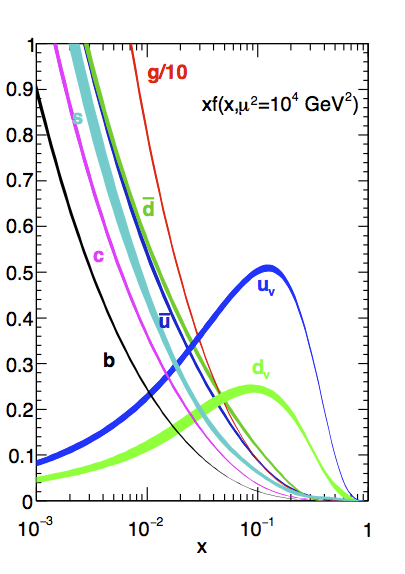
\includegraphics[width=0.65\textwidth]{images/Theory/pdfnob.png}
    \caption{Proton parton distribution functions $xf(x)$ $(f = u_{v},~ d_{v},~ \overline{u},~ \overline{d},~ s\approx\overline{s},~ c\approx\overline{c},~ b\approx\overline{b},~ g$ ) for a given momentum fraction, $x$. Obtained from NNLO NNPDF3.0~\cite{Ball2015}}
    \label{fig:protonPDF}
\end{center}
\end{figure}

Protons in the LHC may a) not interact at all and continue to be accelerated around the ring, b) interact via a soft scatter where the products mostly travel along the direction of the beam, c) participate in a hard interaction where two partons within the protons have a high energy collision in which the products travel transverse to the beam. In the latter case, the remaining partons which have not participated in the hard interaction hadronise and form what is known as the \emph{underlying event} (UE)

\section{Top physics}
The top quark was discovered in 1995 at the Tevatron by the CDF~\cite{PhysRevLett.74.2626} and D0~\cite{Abachi:1995iq} collaborations. It had been hypothesised that there must be a partner to the bottom quark which exists with it in a weak-isospin doublet~\cite{Kobayashi:1973fv}. It is the heaviest quark with a mass approximately equivalent to a lead nucleus. The top quark is the only quark which predominantly decays before it can form any bound states, due to its short lifetime of $5\times10^{-25}$~seconds and hence it is the only quark which can be studied for its spin and polarisation properties. The main decay mode for top quarks is to a bottom quark and a W boson, as shown in Fig.~\ref{fig:tdecay}, which occurs $99.8\pm3.8\textrm{ (exp.)}\pm1.6\textrm {(theo.)} \%$~\cite{2014arXiv1403.7366C} of the time.
 % charged lepton tends to point along the direction of top spin
\begin{figure}[ht!]
\begin{center}
    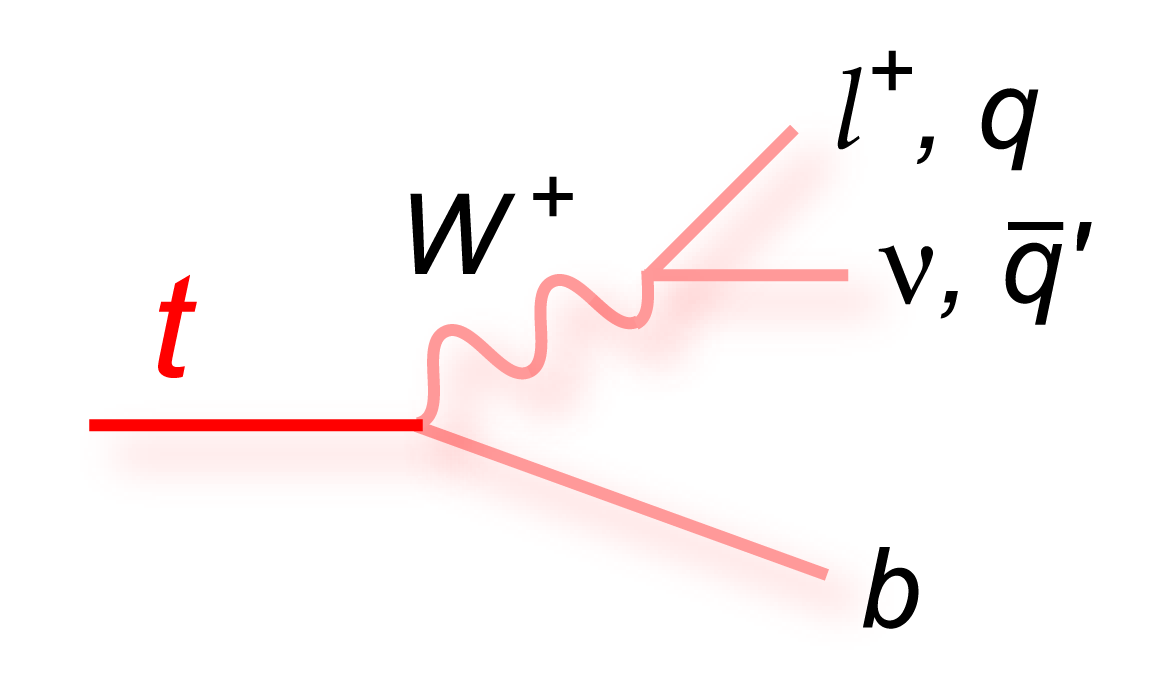
\includegraphics[width=0.49\textwidth]{images/Theory/topdecay.png}
    \caption{Top quark decay to a W boson and b-quark with subsequent decay of the W boson either leptonically or hadronically.}
    \label{fig:tdecay}
\end{center}
\end{figure}

The top quark has the largest Yukawa coupling to the Higgs boson which is of the order of unity. The value of the top quark Yukawa coupling is important in calculations of the stability of the universe and of the energy scales where new physics may arise~\cite{Bezrukov:2014ina}

\subsection{Top pair production}

The first observations of top quarks were made on top pair production (\ttbar) as this is the dominant mechanism for producing top quarks at hadron colliders. Figure~\ref{fig:ttproduction} shows the leading order tree-level production mechanisms via gluon fusion and quark-anti-quark annihilation. 
%The Feynman rules can be used to calculate the amplitude for each diagram and the summation of the amplitudes gives the theoretical cross section at leading order. 

\begin{figure}[ht!]
\begin{center}
    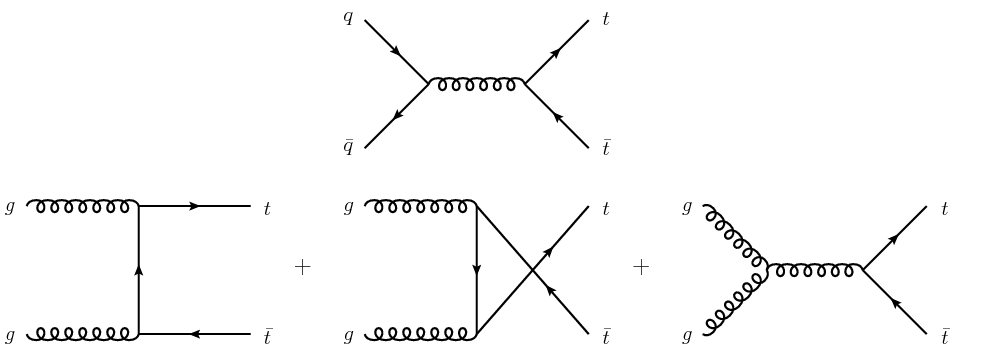
\includegraphics[width=0.95\textwidth]{images/Theory/ttbarfeynman.png}
    \caption{Top quark pair production in the SM by quark-anti-quark annihilation (top) and via gluon fusion (bottom)~\cite{Kohn:2012ksa}}
    \label{fig:ttproduction}
\end{center}
\end{figure}

There are three possible decay modes depending how each top quark decays, as shown in Fig.~\ref{fig:tdecay}: \emph{hadronic} where both W bosons from the top decays decay to a quark and anti-quark, \emph{semi-leptonic} where one W boson decays to \qqbar and one W boson decays to a lepton and a neutrino, and \emph{dileptonic} where both W bosons decay to a lepton and a neutrino each.


\subsection{Single top quark production}

Single top quark production is much rarer than \ttbar production in the SM. It can occur via \qqbar annihilation, g\cPq~fusion or gluon fusion as shown in Fig.~\ref{fig:stFeyn}. In this figure the s-channel (left), t-channel (middle) and associated production with a W boson (tW-channel) are shown.

\begin{figure}[ht!]
\begin{center}
    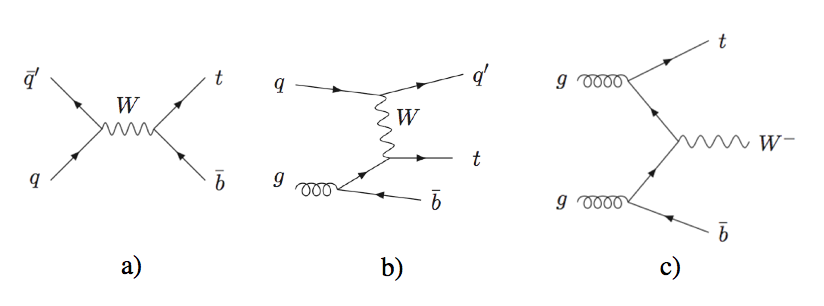
\includegraphics[width=\textwidth]{images/Theory/stFeyn.png}
    \caption{Single top leading order diagrams in the a) s-channel , b) t-channel and c) tW-channel~\cite{Lannon:2012fp}}
    \label{fig:stFeyn}
\end{center}
\end{figure}

The CKM element $|V_{tb}|$ from Eq.~\ref{eqn:CKM2} can be extracted from single top quark decays and the spin of the top quark can be ascertained by studying the leptonic decay of the single top as the charged lepton will point along the direction of the top spin~\cite{Boos:2012hi}.
\subsection{Four top quark production}

The production of four top quarks (\tttt) occurs predominantly via gluon fusion, as seen at leading order in Fig.~\ref{fig:ttttAtLO}, with a $10\%$ contribution from quark-anti-quark annihilation. The production mechanism occurs via QCD whereas the decay of top quarks via W bosons is a weak interaction. 

\begin{figure}[ht!]
\begin{center}
    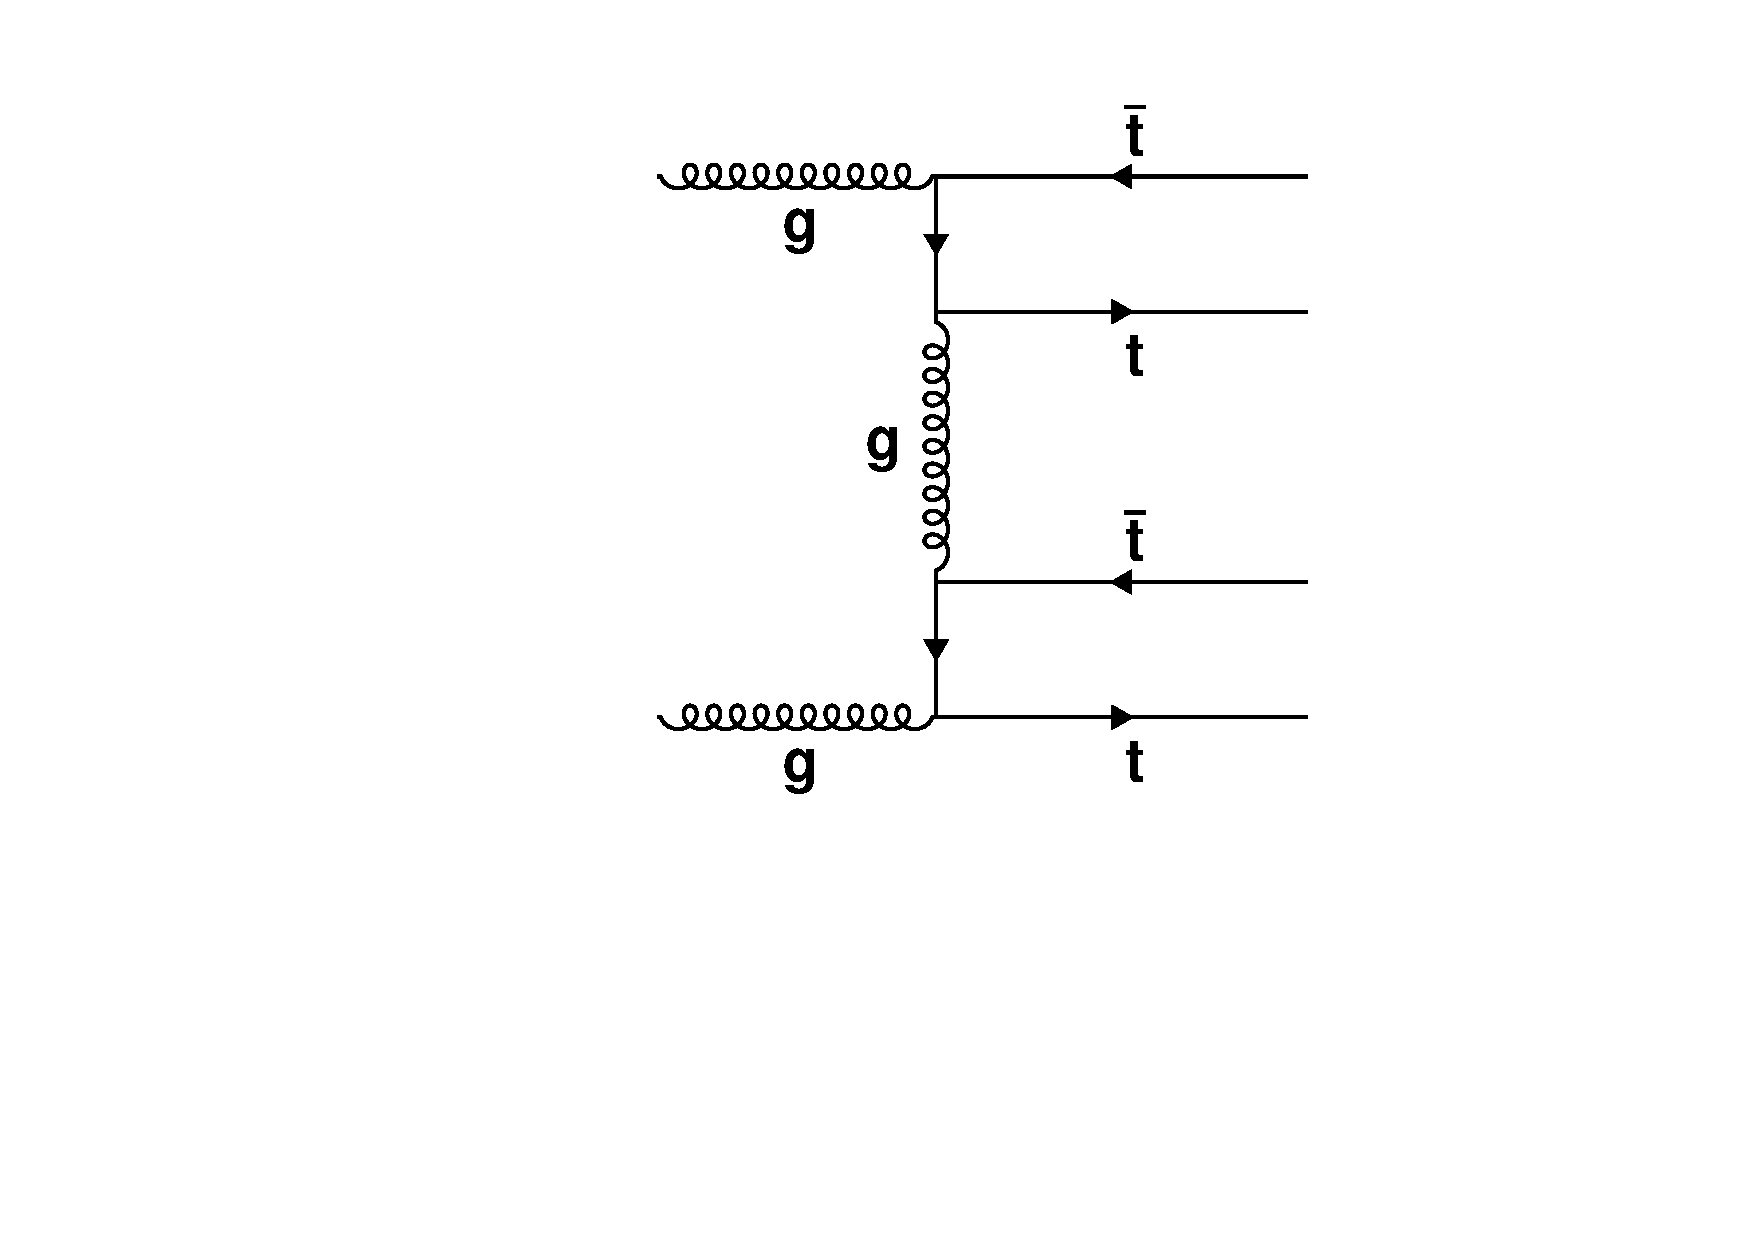
\includegraphics[width=0.49\textwidth]{images/Theory/tttt_t_LO.pdf}
    \caption{Dominant production mechanism for four top quarks in the standard model.}
    \label{fig:ttttAtLO}
\end{center}
\end{figure}

Final states are determined by the decay of the W bosons which can occur either leptonically or hadronically as seen in Fig.~\ref{fig:tdecay}. 


\section{Shortcomings in the standard model ~\label{sec:SMprobs}}
The SM has been resilient to many tests at the LHC, however there are many questions about the universe which the SM cannot answer. For instance:\\
{\bf Gravity :} How can gravity be integrated into the SM and is there an associated boson for the gravitational force~\cite{PhysRevLett.107.171101,PhysRevD.82.122001}? \\
{\bf Matter-anti-matter asymmetry :} How did the matter-anti-matter asymmetry in the universe arise when it is predicted that the number of particle and anti-particles should be conserved in SM interactions~\cite{RevModPhys.76.1}?\\
{\bf Hierarchy problem :} The SM does not provide a solution as to why the Higgs mass is so much smaller than the Planck mass. It also does not describe why the quarks and lepton masses have values which span many orders of magnitude.\\
{\bf Neutrino mass :}
The Sudbury neutrino observatory (SNO) observed that the flux of electron neutrinos from the sun was $\approx 1/3$ what it was expected to be~\cite{PhysRevC.88.025501}. This can be explained by neutrino oscillations. This means that their mass basis is rotated from their flavour basis and hence neutrinos must have mass, which is not part of the SM.\\
{\bf Dark matter :} Observations of the universe show there is non-baryonic, non-luminous matter which is not accounted for within the SM. Studies of galaxy rotation curves show that the angular velocity is relatively constant with radius when it should decrease meaning that there is additional dark matter providing a contribution to the mass of galaxies~\cite{Volders,
Jog:2002dg,
Persic:1995ru}. The presence of dark matter can also be inferred by gravitational lensing. The light from distant stars in the background is curved around the strong gravitational presence of a dark matter cloud, which itself cannot be seen~\cite{Einstein,Ellis2010}. 
This can cause arcs of light and repeated patterns of the same galaxy as seen in Fig~\ref{fig:ttbarAdd}.
\begin{figure}[ht!]
\centering
    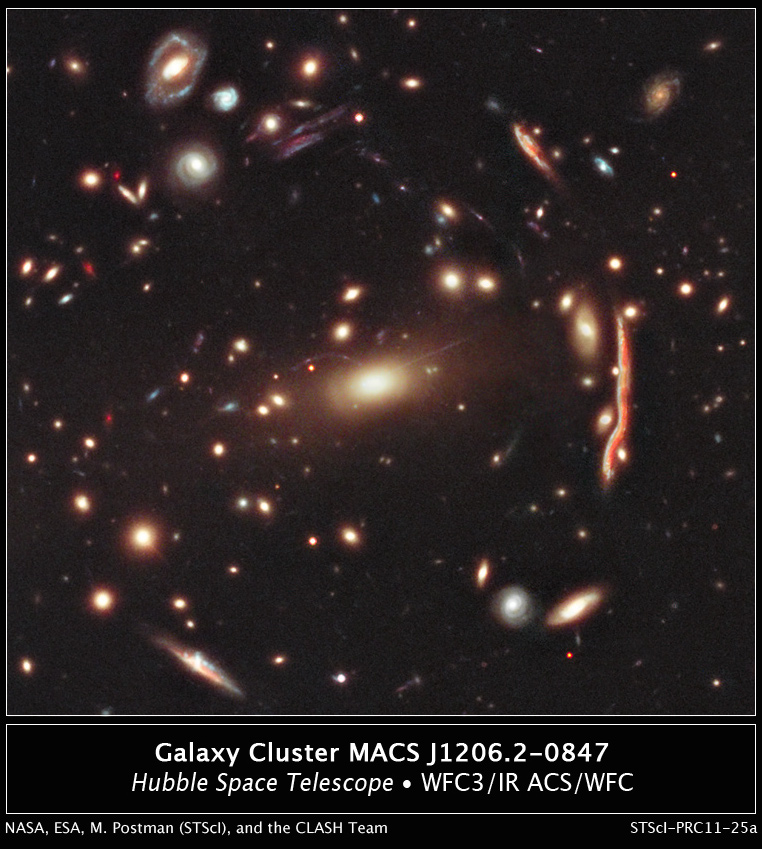
\includegraphics[width=0.65\textwidth]{images/Theory/lensing2.jpg}
    \caption{Gravitational lensing around MACS 1206 as captured by the Hubble Space Telescope~\cite{Glens}}
    \label{fig:Glens}
\end{figure}



\section{BSM models with four top quark signatures ~\label{sec:BSMmodels}}

There are many theories which try to solve some or all of the problems listed in Section~\ref{sec:SMprobs}. Some beyond the standard model (BSM) theories which have final states containing four top quarks are discussed here. 

\textbf{Top quark Compositeness}\\
It has been hypothesised that the top quark could be a composite particle made up of subparticles named preons which are bound by a new confining force. Phenomenological studies have been performed where an effective field theory (EFT) is proposed where only the right-handed top quark is considered to be composite. It is argued that if only $t_{R}$ is composite and no other SM component is then the four top operator will be the most significant component of the EFT lagrangian, which can lead to an enhancement of $\approx 10^3$ to the production of \tttt compared to the SM rate~\cite{Tait2topcomp,Tait1topcomp}.

$\boldsymbol{\ttbar+\textrm{X}, ~\textrm{X}}\rightarrow\boldsymbol{\ttbar}$\\
There are several models which contain \ttbar plus an extra scalar particle which then decays to \ttbar as seen in Fig.~\ref{fig:ttXtt}.
The mediator could be a dark matter mediator~\cite{Arina2016}, a heavy Higgs boson~\cite{Bernreuther:2015fts}, or a member of a scalar colour sextet~\cite{Cacciapaglia2015}, for instance. 

\begin{figure}[ht!]
\centering
    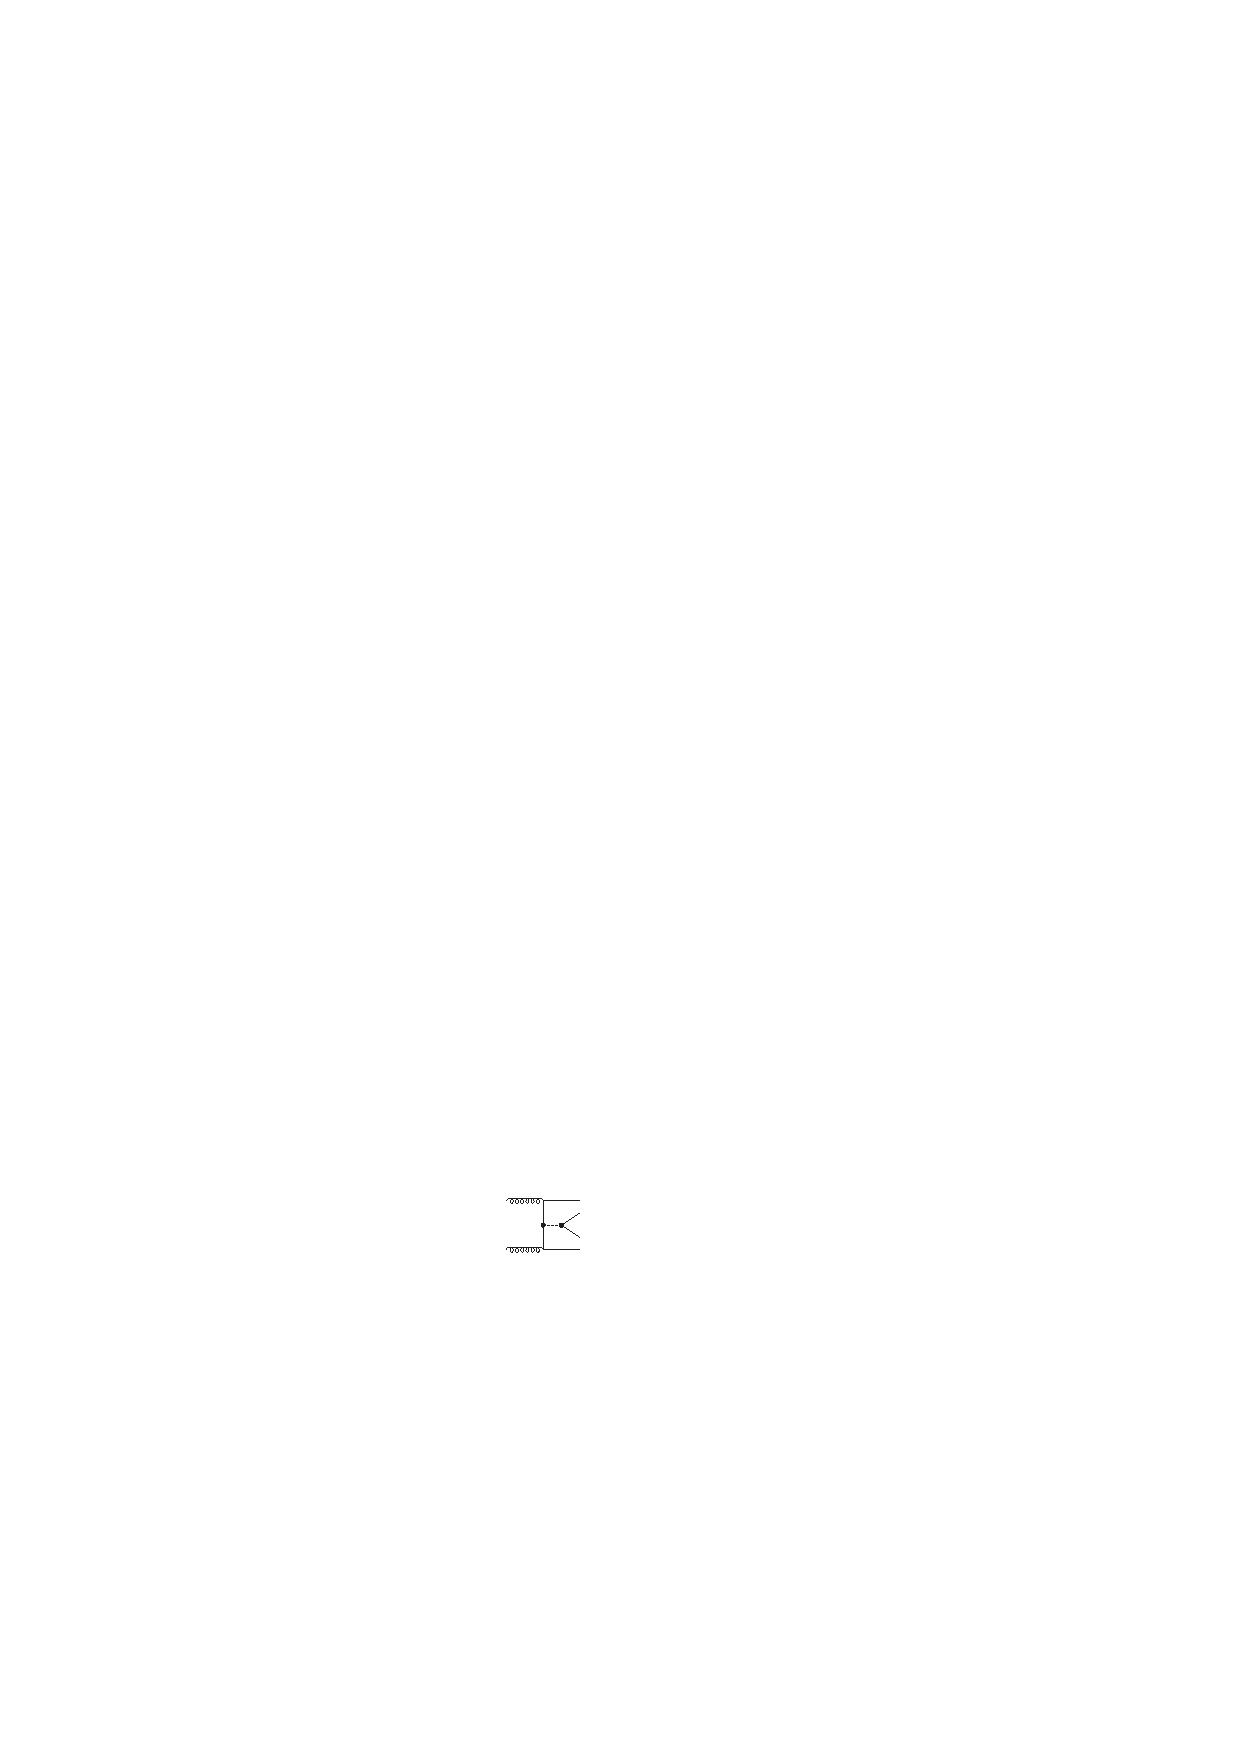
\includegraphics[width=0.45\textwidth]{images/Theory/ttDMtt.pdf}
    \caption{Four top production with an intermediate scalar~\cite{Arina2016}}
    \label{fig:ttXtt}
\end{figure}

% \textbf{Heavy resonances}


\textbf{Scalar pair production to }$\boldsymbol{\tttt}$\\

\begin{figure}[ht!]
\centering
    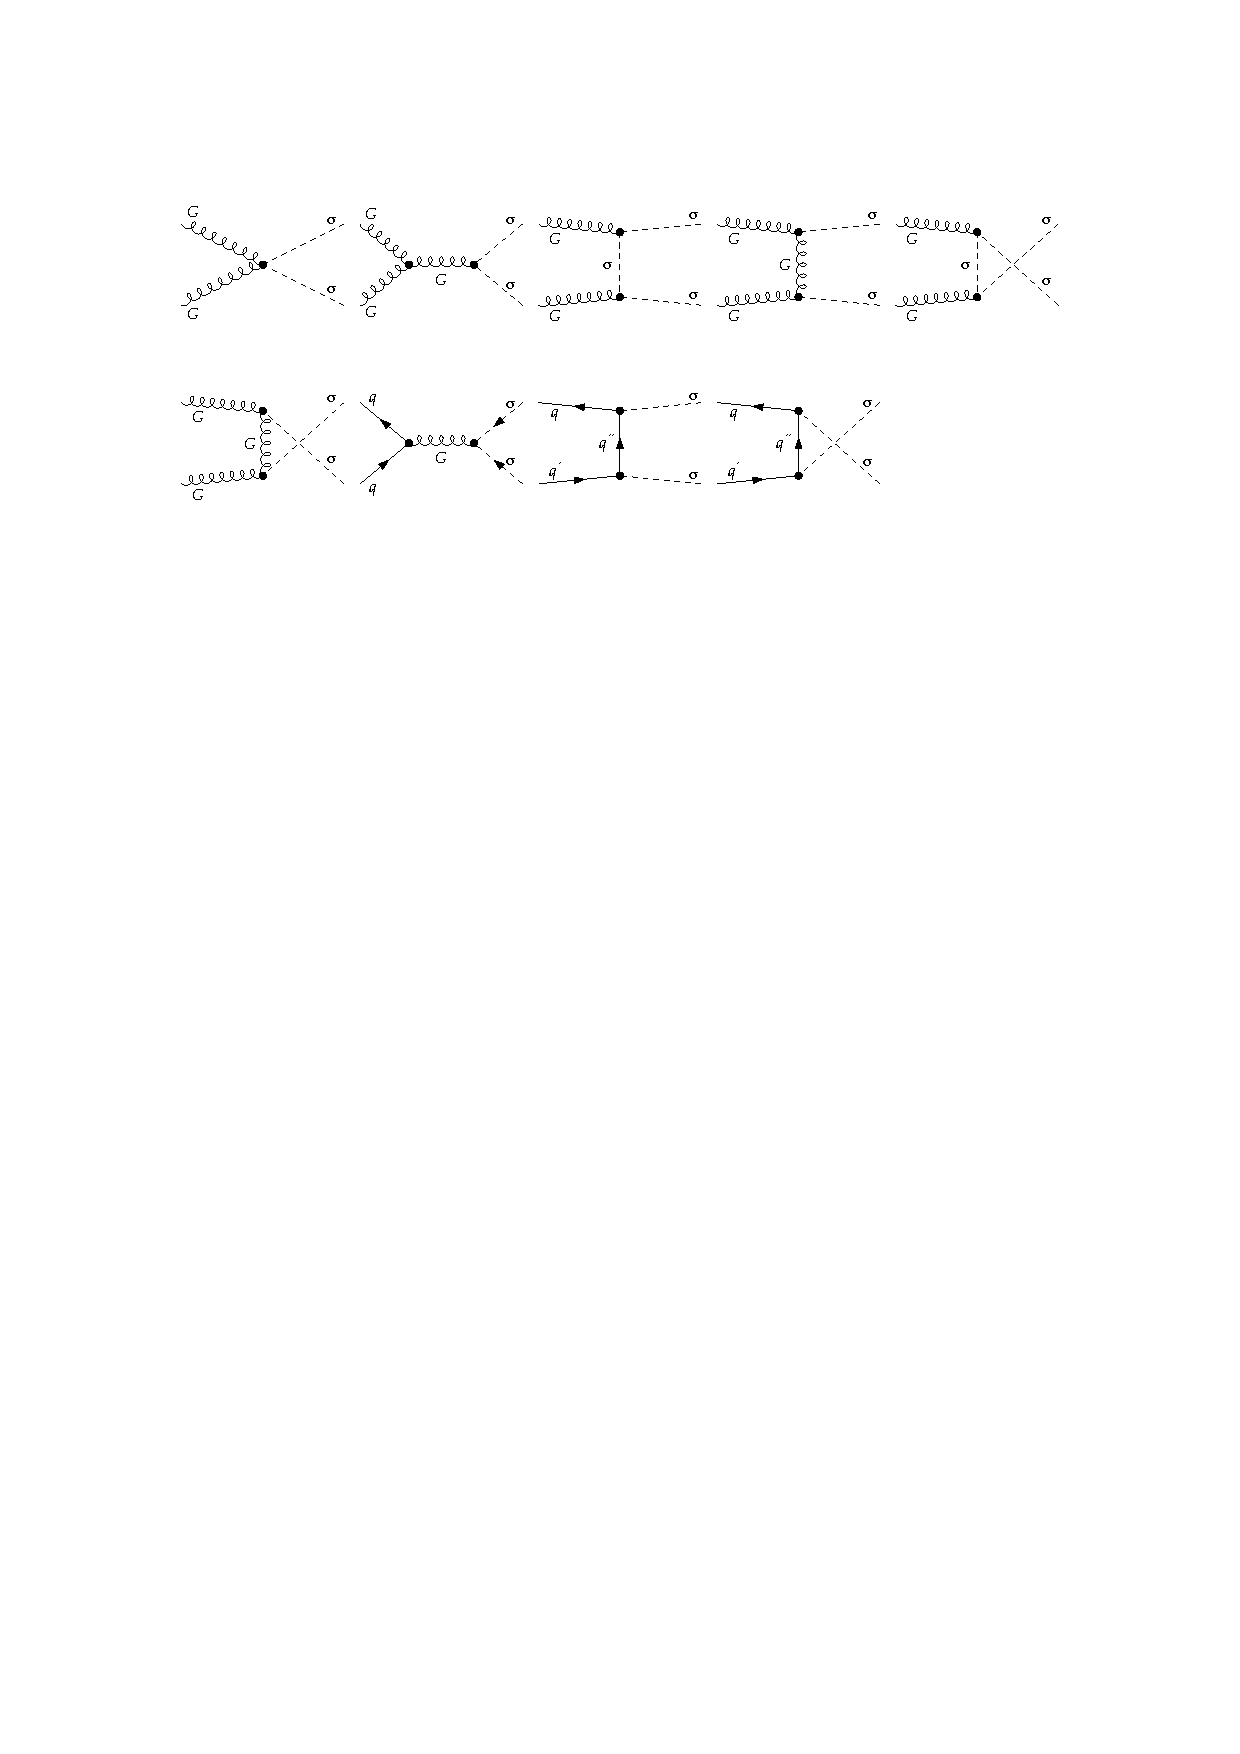
\includegraphics[width=0.99\textwidth]{images/Theory/sgluonFeyn.pdf}
    \caption{Sgluon pair production~\cite{Calvet:2012rk}}
    \label{fig:sgluonpair}
\end{figure}

An additional scalar gluon (\emph{sgluon}) has been theorised in several models of physics beyond the SM. In N=1/N=2 hybrid and R-symmetric versions of non-minimal supersymmetric models (NMSSM) the minimal supersymmetric model (MSSM) is supplemented by an additional chiral multiplet which lies in the adjoint representation of the QCD gauge group. This supermultiplet contains a two-component fermionic part which mixes with the Dirac gluino and a colour-octet complex scalar particle which is the sgluon field. This is particularly interesting because coloured particles will couple directly to gluons and hence should be produced in proton-proton collisions. Figure~\ref{fig:sgluonpair} shows the possible tree level production modes for sgluon pair production.~\cite{Calvet:2012rk}

Sgluons also arise in vector-like confining theories and extra-dimensional models, therefore it is viable to use a simplified model approach (as discussed below) because the final state signatures are reasonably model-independent.

Colour octets and sextets can also be pair produced in theories where the Higgs boson is a composite particle~\cite{Cacciapaglia2015}.



\section{Simplified models}

Simplified models work by building a TeV-scale effective Lagrangian which describes a minimal number of new particles and their interactions. Hence, variables which can be directly observed by the detector can be studied, for example, particle masses, cross sections and branching ratios for different decay modes. Simplified models can sometimes be considered to be a subset of more general physics models where only a few of the particles are considered. Therefore, simplified model cannot be considered to be model independent but they can help to identify the bounds of sensitivity for searches~\cite{0954-3899-39-10-105005}. An example of where a simplified model can be used is in the case of $\ttbar+\textrm{X}$ in Section~\ref{sec:BSMmodels} where the phenomenology of the resulting particles in the detector can be studied without knowledge of which underlying theory the new scalar particle, X, is coming from.


